\documentclass[12pt,a4wide]{report}
\usepackage[latin1]{inputenc}
\usepackage{graphicx}

\def\TitreMemoire{


   Automatisation des tests d'acceptation et int�gration continue: une solution pour r�pondre aux enjeux de l'optimisation de la recette fonctionnelle d'une application

}
\def\AuteurMemoire{Pascal Orsini}
\def\Master{Master MIAGE}

\def\Universite{Universit� Paris-Ouest Nanterre-La D�fense}
\def\Annee{Ann�e Universitaire 2016-2017}

\def\Enseignant{M�moire encadr� par le Pr. Reda Bendraou}


\usepackage[francais]{babel}
\usepackage[T1]{fontenc}
\usepackage{hyperref}
\hypersetup{
colorlinks=true,
linkcolor=black,
citecolor=blue,
filecolor=blue,
urlcolor=blue
}
%\usepackage{fontspec}
%\setmainfont[Ligatures=TeX]{Linux Libertine O}
\usepackage{libertine}

\begin{document}

\thispagestyle{empty}
\begin{center}
\vspace{2cm}
\hrule
\vspace{.5cm}
{\LARGE\textbf{\TitreMemoire}}\\
\vspace{.5cm}
\hrule
\vspace{1cm}
{\Large \AuteurMemoire}\\
\vspace{0,5cm}
{\Large \Master}\\
\vspace{0,5cm}
{\Large \Enseignant}\\
\vspace{8cm}
{\Large \Annee}\\
\vspace{0,5cm}
{\Large \Universite}\\
\vfill
\vspace{2cm}
\end{center}
\newpage

\textbf{Remerciements} 
\bigbreak

Je voudrais tout d'abord exprimer ma profonde reconnaissance � ma tutrice, Dora Toth, ainsi qu'� Ga�tan Cesaro qui ont dirig� mon travail au sein de Veolia Eau d'Ile-de-France tout au long de l'ann�e. La formation qu'ils m'ont offerte m'a permis d'acqu�rir une exp�rience professionnelle solide et riche en apprentissages.

\medbreak

Je souhaiterais �galement remercier l'�quipe avec laquelle j'ai collabor�, notamment Sa�d Maisse, J�r�me Huebra, Thibault Douilly et Guillaume Quenolle qui par leur exp�rience et leur enthousiasme, m'ont apport� une grande aide tout au long de mon ann�e d'alternance.

\medbreak

Je tiens aussi � remercier le corps enseignant de l'Universit� Paris Ouest Nanterre-La D�fense qui m'a suivi durant cette ann�e de formation et m'a fourni l'apprentissage th�orique n�cessaire.
Je remercie tout particuli�rement Monsieur Bendraou et Monsieur Poizat qui ont suivi l'�volution de mon travail et ont largement contribu� �l'am�lioration de mes connaissances.



\tableofcontents
\newpage

\chapter{Introduction}
Au sein des grandes entreprises, le d�veloppement d'une application informatique est organis� autour de trois parties prenantes: le m�tier, la maitrise d'oeuvre et l'assistance � maitrise d'ouvrage. Le m�tier est compos� de collaborateurs au sein du client, qui demeure l'entit� demandeuse du logiciel et qui maitrise le besoin�m�tier auquel ce dernier doit r�pondre. La ma�trise d'oeuvre (MOE) est principalement compos�e de d�veloppeurs et d'architectes logiciels qui auront � charge de r�aliser le logiciel de sa conception technique jusqu'au d�veloppement de l'application. Enfin, l'assistance � ma�trise d'ouvrage (AMOA) est en charge de faire le lien entre les deux�parties. Son r�le consistera principalement � sp�cifier�le besoin du client et de s'assurer que le logiciel d�velopp� par la MOE r�pond aux exigences du m�tier.\medbreak 
Afin de mener sa t�che � bien, la mission de l'AMOA s'articulera autour de nombreux r�les. La premi�re fonction de celle-ci est de�recueillir�le besoin du client. Elle doit pour cela prendre connaissance de mani�re pr�cise du besoin m�tier auquel le logiciel devra r�pondre. � partir de ce recueil de besoin, l'AMOA r�digera les sp�cifications fonctionnelles de l'application qui consistent en une explication pr�cise du workflow de l'ensemble des fonctionnalit�s propos�es par le logiciel. \medbreak 
En outre, durant chacune des �tapes du d�veloppement, l'AMOA doit s'assurer que le logiciel correspond � ce qui est attendu par le m�tier en suivant son �volution mais aussi en effectuant diff�rents tests lors de chacune des livraisons: les tests d'acceptation et les tests de non r�gression. En�effet, un�des r�les primordiaux de l'assistance�� maitrise d'ouvrage consiste � r�aliser la recette logicielle. Cette�derni�re�d�signe une vaste campagne de tests permettant de valider la livraison d'un programme mais aussi de d�tecter les bugs, aussi bien sur le plan technique que fonctionnel � travers un grand nombre de�tests effectu�s directement au sein de l'application qui permettront leur d�tection.\medbreak 
Les tests de non-r�gression�consistent � tester l'application afin de s'assurer que l'avanc�e dans le d�veloppement, la livraison de correctifs ou de mises � jour ne soit pas source d'anomalies concernant des fonctionnalit�s parfaitement op�rationnelles jusqu'alors. Ces tests sont primordiaux car la r�gression est synonyme de perte de temps au sein du processus de d�veloppement logiciel de par le ralentissement de l'avanc�e du travail dont elle peut �tre � l'origine. En effet, elle peut obliger la MOE � se consacrer � des fonctionnalit�s qui �taient consid�r�es comme �tant valid�es. Les tests de non-regression doivent donc �tre effectu�s de mani�re r�guli�re et�apr�s chacune des livraisons afin de s'assurer que le comportement du logiciel est en ad�quation avec ce qui est attendu. Ceux-ci�doivent ainsi�couvrir les fonctionnalit�s aussi bien anciennes que nouvelles de l'application afin de s'assurer qu'elles ne subissent pas d'alt�ration de comportement. Ainsi, en fonction de la taille d'une application, il peut exister un grand nombre de tests de non-r�gression �effectuer apr�s chaque livraison. R�aliser l'ensemble des tests de non-r�gression de mani�re r�guli�re�peut repr�senter une charge de travail lourde et fastidieuse, notamment si la fr�quence des mises � jour est �lev�e. \medbreak 
L'objectif de ce m�moire est de comprendre les enjeux de l'automatisation de la recette fonctionnelle au sein du cycle de d�veloppement logiciel. Nous commencerons par�pr�senter le contexte de d�veloppement d'un logiciel au sein d'une entreprise, c'est-�-dire les diff�rentes phases cl�s qui le�compose, tout en se focalisant principalement sur le test logiciel. Nous�effectuerons ensuite un �tat de l'art au sein duquel nous comparerons les diff�rents outils permettant de mettre en place une automatisation de la recette fonctionnelle existant sur le march�. Enfin, dans une troisi�me et derni�re partie, nous�proposerons une solution permettant d'am�liorer la�d�tection�de�r�gressions�durant le processus de livraison de mise � jour en mettant en place un pipeline comprenant des tests Selenium au sein de l'outil d'int�gration continue�Jenkins. \medbreak

\chapter{Contexte et probl�matique}
\section{Le cycle de vie d'une application}

Le cycle de vie d'un logiciel est constitu� de diff�rentes phases:
\begin{itemize}  
\item Sp�cification g�n�rale de l'application
\item Sp�cification fonctionnelle 
\item Sp�cification technique 
\item D�veloppement 
\item Int�gration 
\item Mise en production 
\item Maintenance 
\end{itemize}
\medbreak

La sp�cification g�n�rale est la premi�re �tape du cycle de vie du logiciel. C'est durant cette �tape que seront d�finis les besoins auxquels l'application devra r�pondre. Cette phase est principalement r�alis�e par le m�tier qui sera en charge d'effectuer le premier cadrage du logiciel. \newline 
La seconde phase, l'�criture des sp�cifications fonctionnelles, aura pour but de d�finir la partie fonctionnelle de l'application. Il s'agit d'une description pr�cise des fonctionnalit�s de l'application, elle explicite la mani�re avec laquelle cette derni�re r�pondra aux besoins du m�tier. C'est durant cette phase que sera seront sp�cifi�s les diff�rents workflow d'utilisation du logiciel par les utilisateurs ainsi que les diff�rentes interfaces qui seront impl�ment�es. \newline
La sp�cification technique d�crit le fonctionnement de l'application d'un point de vue technique: architecture, infrastructure ou encore gestion des donn�es utilis�es. C'est durant cette phase que sera effectu� le choix de l'ensemble des outils de couvrir l'ensemble du cycle de vie de l'application, de la cr�ation jusqu'� sa mise en production. 
\newline
La phase de d�veloppement est la phase pendant laquelle l'application est cod�e par la ma�trise d'oeuvre. Durant cette phase, l'AMOA suit le travail de la MOE afin de veiller � ce que l'application r�ponde de mani�re pr�cise au besoin du client. \newline
L'int�gration demeure la phase durant laquelle les diff�rents composants de l'application sont rassembl�s les uns avec les autres dans le but d'effectuer la v�rification du bon fonctionnement de l'ensemble. \newline
La mise en production est la phase o� l'application est mise � la disposition du client. L'application sera alors en phase de maintenance, phase durant laquelle sera assur� le maintien de l'application en condition op�rationnelle. En effet, apr�s une mise en production, une application conna�tra r�guli�rement des mises � jour en fonction des retours du client mais aussi pour correspondre � des �volutions des besoin pouvant subvenir ult�rieurement. \medbreak

\begin{figure}[!h] 
\centerline{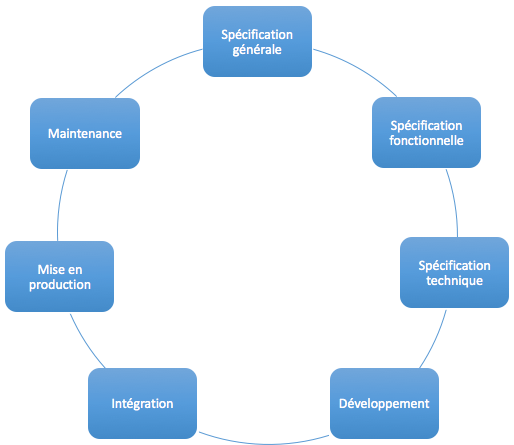
\includegraphics[scale=0.65]{cyclevie.png}}
\caption{Le cycle de vie d'une application}
\end{figure} 


Ces phases peuvent n�cessiter des allers-retours entre elles car les besoins m�tiers peuvent �voluer et n�cessiter une mise � jour des sp�cifications r�alis�es jusqu'alors. De plus, il est possible qu'une application soit livr�e par lot, certaines fonctionnalit�s deviennent alors accessibles au fur et � mesure des livraisons. Dans ce cas, certaines �tapes peuvent �tre effectu�es en parall�le. Par exemple, la sp�cification fonctionnelle du lot 2 est r�alis�e pendant que le lot 1 est en phase de d�veloppement.

\section{La recette fonctionnelle}

La r�alisation de la recette fonctionnelle est bas�e sur l'ensemble des sp�cifications fonctionnelles r�dig�es par l'assistance � maitrise d'ouvrage. Il s'agit de proc�der � l'int�gralit� des tests d'acceptation utilisateur afin de s'assurer que l'ensemble des fonctionnalit�s livr�es sont en ad�quation avec ce qui est d�fini par le m�tier au sein des sp�cifications globales de l'application. Chacun des cas d'utilisation du logiciel doit donc �tre couvert par la recette fonctionnelle. Il s'agit d'une �tape extr�ment importante car le co�t g�n�r� par la correction d'une erreur d'exigence pour une entreprise peut �tre de 50 � 200 fois sup�rieur si celle-ci est effectu�e lors de la maintenance de l'application que si elle avait eu lieu lors de la phase de d�veloppement\cite{1}. \newline

\subsection{L'environnement de recette}
Tout au long du d�veloppement d'une application, celle-ci se trouve distribu�e au sein de plusieurs environnements. G�n�ralement, c'est autour de cinq environnements que la distribution de l'application s'op�re:
\medbreak

\begin{itemize}  
\item D�veloppement 
\item Int�gration 
\item Recette 
\item Pr�-production
\item Production  
\end{itemize}

\medbreak
L'environnement d�veloppement est celui sur lequel s'effectue directement le d�veloppement. C'est au sein de cet environnement que travaillent principalement les diff�rents d�veloppeurs. L'environnement int�gration est celui au sein duquel les diff�rents composants de l'application sont assembl�s. L'environnement recette est celui o� est publi�e la livraison d'une mise � jour afin de la mettre � disposition de l'AMOA qui pourra alors effectuer les tests fonctionnels et de non-regression. C'est au sein de cet environnement que l'on pourra donc valider, ou non, une livraison logicielle. L'environnement de pr�-production est similaire � l'environnement recette sauf que l'architecture serveur de cet environnement est identique � l'architecture de l'environnement de production afin de reproduire le comportement exact de l'application utilis�e par le client. Enfin, l'environnement de production est l'environnement au sein duquel l'application est accessible aux utilisateurs. La livraison sur cet environnement demeure l'�tape finale de la livraison d'une mise � jour. 
\medbreak

\begin{figure}[!h] 
\centerline{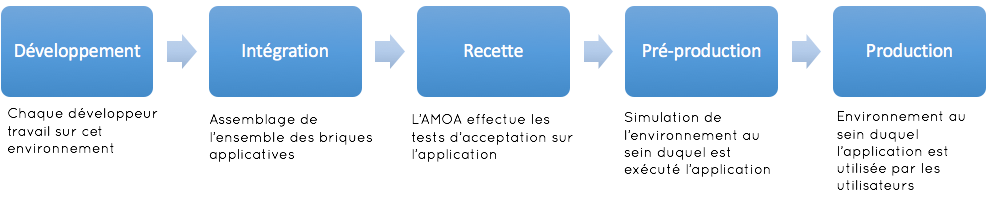
\includegraphics[scale=0.50]{environnements.png}}
\caption{Les environnements utilis�s pour le d�veloppement d'une application}
\end{figure} 
\medbreak


\subsection{Les cahiers de recettes}
Pour effectuer des tests d'acceptation et de non-r�gression, il est imp�ratif de proc�der � l'�tablissement de cahiers de recettes. La recette de chacune des mises � jour permettra de d�tecter les�r�gressions.�Celle-ci s'effectuera sur l'environnement de recette. Chaque�d�but de phase de tests commence par la lecture de la sp�cification associ�e � la fonctionnalit� � tester ainsi qu'� la prise de connaissance du cahier de recette associ�. Bien comprendre les sp�cifications est indispensable au bon d�roulement de la recette car cela permet de clairement conna�tre le comportement � attendre de l'application et d'�tre certain de bien identifier les�erreurs.�En outre, lorsqu'ils sont effectu�s avant une premi�re livraison de fonctionnalit�, les tests d'acceptation permettent de s'assurer que l'application d�velopp�e respecte bien les informations comprises au sein des sp�cifications fonctionnelles �crites par l'AMOA. \medbreak
Les tests d'acceptation�n�cessitent�de se positionner en tant qu'utilisateur de l'application et d�rouler les sc�narios d'utilisation du logiciel d�crit dans le cahier de recette. Il est important de�mettre�� jour ces m�mes cahiers lors de chaque livraison de nouvelles fonctionnalit�s car celles-ci�devront �tre � leur tour test�es lors de livraisons ult�rieures.�Chacun des sc�narios de test doit permettre de v�rifier que l'application adopte le comportement d�crit au sein des sp�cifications. La structure des cahiers de�recette�est la suivante:�
\medbreak
\begin{itemize}  
\item Cas de test� 
\item Action � effectuer 
\item R�sultat attendu
\item R�sultat obtenu  
\end{itemize}
\medbreak
Le cas de test d�signe le contenu du test qui va �tre r�alis�, c'est-�-dire la fonctionnalit� qui va �tre test�e. Il existe deux types de cas de tests, les cas de tests passants, qui d�signent des tests�qui doivent se r�v�ler positifs�pour��tre�consid�r�s�comme�r�ussi�ou bien les cas de tests non-passants qui doivent, eux, �chouer. Ces derniers concernent par exemple le cas d'une situation qui ne doit pas��tre�possible, comme l'acc�s � certaines donn�es, ou la possibilit� d'effectuer une action qui ne doit pas �tre r�alisable au sein de l'application.��\medbreak
L'action � effectuer explique les diff�rentes �tapes � r�aliser afin d'ex�cuter le test, les pr�requis n�cessaires, les donn�es � renseigner au sein de l'application ou encore d'�tre�connect� avec un utilisateur ayant, ou non, les droits pour utiliser la fonctionnalit� en question. Le r�sultat attendu est le comportement que l'on attend de l'application suite � l'action effectu�e. Si le comportement est conforme aux attentes, le r�sultat obtenu sera consid�r� comme positif, si le comportement est contraire, il sera consid�r� comme n�gatif.    \medbreak

\subsection{L'automatisation de la recette fonctionnelle}
Selon B�rge Haugset et Geir Kjetil Hanssen \cite{2}, effectuer manuellement les tests d'acceptation constitue une t�che fastidieuse, co�teuse et consommant beaucoup de temps. L'automatisation de ces tests peut donc sembler �tre une initiative prometteuse pour faciliter et am�liorer ce processus.
N�anmoins, l'automatisation des tests peut n�cessiter 3 � 10 fois le temps n�cessaire � la cr�ation et � l'ex�cution d'un test manuel \cite{3}. Ainsi, sur un tr�s court terme, il s'agit effectivement d'un tr�s fort co�t � supporter pour l'entreprise, car la mise en place de tests automatis�s n�cessite beaucoup de temps pour �tre mise en place. Cependant, si ces tests automatis�s sont r�utilisables sur une longue dur�e, cet investissement initial peut permettre d'�conomiser les co�ts pour une entreprise � long terme. C'est pourquoi il demeure important de d�terminer les tests qui m�ritent d'�tre automatis�s \cite{4}. Un autre avantage de l'automatisation de la recette fonctionnelle r�side dans le fait que celle-ci peut �tre effectu�e avec une fr�quence d'ex�cution largement sup�rieure car elle peut �tre lanc�e � chaque instant \cite{5}. En outre, l'automatisation des cas de tests engendre une r�elle fiabilit� car, une fois les test valid�s, ils ne peuvent pas �chouer. Si un �chec est rencontr�, il est obligatoirement d� � une regression ou une anomalie au sein de l'application.

\section{L'int�gration continue au service de la recette fonctionnelle}
L'int�gration continue consiste en un ensemble de pratiques en vigueur au sein du processus de d�veloppement d'une application visant � s'assurer que chacune des modifications effectu�es au sein du code source n'est pas � l'origine de r�gression au sein de celle-ci. Cet ensemble de pratiques d'ing�nierie logicielle va permettre d'acc�l�rer la livraison des applications en r�duisant les temps d'int�gration \cite{6}. Pour ce faire, l'int�gration continue repose sur trois points cl�s \cite{7}:

\begin{itemize}  
\item La centralisation: l'int�gralit� du code est centralis� sur le serveur d'int�gration continue.
\item L'automatisation: les builds, les d�ploiement ainsi que les tests sont effectu�s automatiquemment.
\item L'historisation: les anciennes versions sont stock�es et accessibles sur le serveur, permettant ainsi de comparer les �volutions de l'application.
\end{itemize}
\medbreak

Un des enjeux de l'int�gration continue est similaire � un enjeux de la recette fonctionnelle: �tre inform� en cas d'anomalie pr�sente ou de regression survenue au sein de l'application. La recette �tant effectu�e par l'AMOA et l'int�gration continue par la MOE, il peut ainsi s'av�rer int�ressant pour une entreprise de lier le travail des deux corps de m�tier en int�grant la recette fonctionnelle au sein de l'int�gration continue. En effet, ce lien permettrait � la MOE de d�tecter rapidement les regressions fonctionnelles lors de chacuns des builds automatis�s effectu�s via le serveur d'int�gration continue.

\section{Les enjeux de la recette fonctionnelle}

Effectuer une recette compl�te sur l'environnement de recette ou de pr�-production est imp�ratif avant chaque livraison de fonctionnalit� ou de mise � jour effectu�e sur l'environnement de production. Si ces derni�res ont lieu r�guli�rement, la recette peut n�cessiter une charge de travail cons�quente. Cette �tape demeurant incontournable lors de la livraison d'une application, par quels moyens peut-on am�liorer son d�roulement ainsi que son efficacit�? Comment int�grer cette �tape cl� du processus de livraison au sein de l'int�gration continue mise en place par les �quipes de d�veloppement? \newline
�\medbreak

\chapter{\'Etat de l'art}
Il existe actuellement un grand nombre d'applications permettant d'effectuer des tests fonctionnels bas�s sur l'interface utilisateur. Chacun d'entre eux dispose d'avantages et d'inconv�nients en fonction de l'utilisation souhait�e. La grande force de ces applications demeure dans le fait qu'elles sont capables de simuler les actions d'un utilisateur sur une application afin de v�rifier son bon fonctionnement. Ainsi, elles permettent de d�tecter les r�gressions fonctionnelles de mani�re automatique et sans intervention humaine une fois que les tests ont �t� mis en place. Elles peuvent ais�ment �tre � l'origine de gain de temps au sein du cycle de d�veloppement d'une application car elles d�tectent imm�diatement les r�gressions suite � une livraison. \medbreak

En outre, l'utilisation d'un outil d'int�gration continue est devenue au fil du temps un �l�ment cl� au sein du processus de d�veloppement logiciel. L'objectif de l'int�gration continue est de s'assurer que chaque modification effectu�e au sein du code de l'application n'est pas source de regression ou d'erreurs (lors du build de l'application, de son d�ploiement ou bien lors de l'ex�cution de tests par exemple). 

\section{Les outils d'automatisation des tests}
\subsection{Selenium IDE}


Selenium IDE est une extension pour le navigateur web Mozilla Firefox permettant d'ex�cuter des scripts Selenium \cite{8}. Il permet de proc�der � l'enregistrement et la cr�ation de scripts permettant d'effectuer des tests fonctionnels sur une application web. Le principe de fonctionnement est extr�mement simple, Selenium IDE r�cup�re les XPath des �l�ments qui composent une page web et utilise ces �lements selon le souhait de l'utilisateur lors de l'�criture du script. \medbreak
\begin{figure}[!h] 
\centerline{
\includegraphics[scale=0.70]{seleniumLogo.png}}
\caption{Selenium IDE}
\end{figure} 

Selenium IDE est tr�s simple � prendre en main gr�ce � sa fonction enregistreur qui consiste � enregistrer les actions effectu�es par la souris et le clavier de l'utilisateur. Ces tests peuvent �galement �tre cr��s � l'aide de commandes incluses au sein de l'application qui permettent de simuler le comportement d'un utilisateur avec l'application. En effet, la fonction d'enregistrement atteint vite ses limites car on ne peut pas simuler l'attente du chargement d'un �l�ment de la page, Selenium d�clarant le test echou� d�s lors qu'il ne trouve pas un �l�ment, un chargement un peu long d� � une lenteur sur un serveur aura comme effet de faire �chouer le test. Ainsi, l'insertion d'une commande "WaitForElementPresent" permettra d'informer Selenium que celui-ci doit attendre que l'�l�ment soit charg� par l'application afin de continuer la simulation du comportement utilisateur, chose impossible un utilisant uniquement la fonction enregistreur d'�v�nements. Les scripts Selenium IDE peuvent �galement �tre �crits en Java, C\# ou Python.
\newline
Autre fonctionnalit� int�ressante de Selenium, celui-ci dispose d'un outil de planification de l'�xecution automatique des tests. Ainsi, ces derniers peuvent s'ex�cuter automatiquement � la date et l'heure choisie par l'utilisateur avec la possibilit� d'impl�menter une r�currence pour l'ex�cution des tests.\newline
\newpage

Exemple de commandes propos�es par Selenium :\newline \medbreak
\begin{tabular}{|p{6,2cm}|p{6,2cm}|}

  \hline
  Commande & Description� \\
  \hline
  open & Ouvre un URL dans la fen�tre du navigateur en cours  \\ \hline
  waitForElementPresent�& Attend qu'un �l�ment HTML soit pr�sent dans la page. Permet de v�rifier que la page est charg�e avec l'�l�ment d�sir� \\ \hline
  click�& Simule un clic sur un �l�ment HTML   \\ \hline
  assertText�& V�rifie la pr�sence d'une chaine de caract�re \\ \hline
  select &  S�lectionne un �l�ment dans une liste    \\ \hline
  pause & Met le test en pause selon une dur�e choisie� \\ \hline
  close & Ferme un onglet  \\ \hline
  store & Permet de stocker une valeur au sein d'une variable  \\ 
  \hline
\end{tabular}
\medbreak \medbreak
Ces commandes sont regroup�es au sein d'un script qui sera le test ex�cut�: \newline\medbreak
\begin{tabular}{|p{4cm}|p{4cm}|p{4cm}|}
  \hline
  Commande & Cible de l'application� & Valeur \\ 
  \hline
  open & Url de l'application &  \\ \hline
  waitForElementPresent�& XPath de l'�lement�& XPath de l'�lement \\ \hline
  click� & XPath de l'�lement &  \\ \hline
  assertText�& XPath de l'�lement & Texte qui doit �tre trouv� \\
  \hline
\end{tabular}
\medbreak
\medbreak
Selenium IDE est donc un outil tr�s simple � utiliser mais qui souffre d'un d�faut majeur, il n'arrive pas � travailler avec les pages web dynamiques cr��es avec Javascript ou Ajax. Par exemple, une application javascript monopage posera de serieux probl�mes � Selenium car celui-ci peut confondre deux �lements pourtant diff�rents visuellement pour l'utilisateur, mais avec des similarit�s au niveau du code source exploit� par Selenium.
\medbreak

Il existe une seconde version de Selenium, Selenium WebDriver. Cette version est une API Java qui pr�sente l'avantage de pouvoir utiliser des listeners ou bien d'effectuer des tests sur des applications mobile. L'utilisation de la fonction d'enregistrement est par contre inutilisable avec cette version.

\subsection{Sikuli}
\begin{figure}[!h] 
\centerline{
\includegraphics[scale=0.40]{sikuliLogo.png}}
\caption{Sikuli}
\end{figure} 

Sikuli est une application permettant d'automatiser des actions sur l'interface graphique d'un ordinateur. Contrairement � Selenium qui n'interagit qu'avec un navigateur web, Sikuli est capable d'agir sur l'int�gralit� du syst�me \cite{9}. En effet, il peut effectuer des t�ches telles que le lancement d'une application par exemple la ou Selenium n�cessite d'avoir le navigateur d�j� lanc� et se limite aux tests sur ce navigateur.\medbreak
Le fonctionnement de Sikuli est assez similaire � celui de Selenium IDE, la principale diff�rence r�side dans le fait de s�lectionner des images pour alimenter les scripts. En effet, la barre d'outil de l'IDE contient un bouton "Prendre une capture d'�cran" qui permet � l'utilisateur de s�lectionner un �l�ment de l'application sur lequel Sikuli agira.\medbreak
Tout comme Selenium IDE, il est possible de cr�er des script Sikuli � l'aide de langage de programmation tel que Python, Ruby ou encore Java. En revanche, il ne dispose pas de fonction permettant de planifier l'ex�cution des tests.


\subsection{Kantu Web Automation}
\begin{figure}[!h] 
\centerline{
\includegraphics[scale=1]{kantuLogo.png}}
\caption{Kantu Web Automation}
\end{figure} 


Kantu Web Automation est une solution qui constitue un serieux concurrent de Selenium IDE et de Sikuli. Il s'agit d'une application bas�e sur les images, � l'instar de Sikuli, mais aussi des actions de l'utilisateur, � l'instar de Selenium IDE. \cite{10} \medbreak 
Tout comme ces deux applications, il est possible de cr�er des scripts dans diff�rents langages tels que Java, C\# ou encore Python mais cela n�cessite l'achat de la version payante de l'application. En effet, la version gratuite offre uniquement la possibilit� d'utiliser la fonction enregistrement ou bien d'ins�rer les commandes manuellement une � une. Kantu Web Automation demeure donc une alternative int�ressante mais peut s'av�rer limit� sans acqu�rir la version payante. 


\subsection{Sahi}

\begin{figure}[!h] 
\centerline{
\includegraphics[scale=0.95]{sahiLogo.png}}
\caption{Sahi}
\end{figure} 

Sahi est un outil disponible en deux versions, une est open source et gratuite, l'autre payante et propri�taire. La version gratuite est assez similaire � ce que propose la concurrence de par les fonctionnalit�s propos�es. La version payante de Sahi se diff�rencie des autres outils en proposant aux utilisateurs la possibilit� d'�xecuter diff�rents tests en parral�lle sur diff�rents navigateurs, le stockage des r�sultats des tests effectu�s au sein d'une base de donn�es afin de pouvoir effectuer un suivi des r�sultats obtenus mais aussi un framework Excel \cite{11}. \medbreak
Ce framework est une des principales forces de Sahi. Celui-ci permet en effet d'�crire des cas de tests en renseignant simplement un tableau dans un document Excel. Ainsi, il demeure tr�s simple pour un non initi� de mettre en place une automatisation des tests avec cet outil et l'int�gralit� des tests r�dig�s peuvent �tre stock�s au sein d'un document Excel. Les tests doivent �tre renseign�s dans un tableau contenant au minimum trois colonnes: TestCase, Keyword et Argument, chaque ligne du tableau constituera une action � effectuer par l'outil. La colonne TestCase est renseign�e afin de sp�cifier le d�but d'un cas de test, elle n'est utilis�e que si le tableau contient plusieurs cas de test et comporte uniquement le nom du cas de test en question. La colonne Keyword contient l'action � effectuer par Sahi au sein de l'application. La colonne Argument contient des donn�es qui doivent �tre utilis�es si besoin est, comme par exemple une valeur � renseigner ou � sauvegarder. Il est possible d'ajouter plusieurs colonnes d'argument au sein du tableau Excel.

\subsection{HP - Unified Functional Testing}
\begin{figure}[!h] 
\centerline{
\includegraphics[scale=0.50]{hpuftLogo.png}}
\caption{HP - Unified Functional Testing}
\end{figure} 

HP - Unified Functional Testing est le logiciel d'automatisation de tests d'acceptation fourni par la soci�t� am�ricaine Hewlett-Packard \cite{12}. Il s'agit d'un outil extr�mement complet, permettant d'effectuer des tests sur les applications web mais aussi sur les smartphones Android, Windows Mobile et iOS. Ces tests peuvent �galement �tre effectu�s en parall�le � travers diff�rents navigateurs pour la version web de l'application d�velopp�e mais aussi entre la version web et la version mobile de l'application, que cette derni�re soit native ou non. En outre, HP - Unified Functional Testing peut aussi effectuer des tests directement au sein des principaux ERP tel que SAP ou des CRM comme Salesforce par exemple. Il peut donc �tre utilis� pour effectuer des tests d'acceptation ou de non-regression sur un panel plus large d'applications. \newline
HP - Unified Functional Testing demeure une solution compl�te mais on�reuse. En effet, l'outil peut co�ter plus de 2000� par an et par poste utilisateur ce qui peut diriger les entreprises vers des alternatives gratuites ou au prix moins �lev�.

\section{Les outils d'int�gration continue}

De nombreux outils d'int�gration continue sont disponibles sur le march�. Parmis eux, on peut notamment citer Jenkins, Travis CI, Bamboo ou encore Circle CI. Les outils d'int�gration continue sont install�s sur des serveurs et permettent d'effecuter l'automatisation de t�ches telles que le d�ploiement, le build ou encore le test d'une application. \medbreak 

\begin{figure}[!h] 
\centerline{
\includegraphics[scale=0.60]{integLogo.png}}
\caption{Des nombreux outils d'int�gration continue sont disponibles sur le march�}
\end{figure} 

Jenkins est un outil d'int�gration continue open-source orient� projet Java \cite{13}. Jenkins est un fork, c'est � dire une nouvelle application cr��e � partir du code source d'une autre application, de l'outil Hudson. Ce dernier constitue un outil similaire � Jenkins mais n'est pas open-source, il appartient en effet � l'entreprise Oracle. La derni�re version stable publi� de Jenkins date du 26 Avril 2016, l'outil demeure mis � jour de mani�re r�guli�re. C'est lors de la sortie de la version 2.0 en 2016 que Jenkins int�gre le pipeline as code en son sein. \medbreak
Bambou est l'outil d'int�gration continue d�velopp� par la soci�t� Atlassian. Cette soci�t� est aussi connue pour la r�alisation des applications Jira, Bitbucket ou encore Trello \cite{14}. Ainsi, Bamboo est con�u pour fonctionner en parfaite harmonie avec les autres logiciels fourni par Atlassian. Il pr�sente ainsi l'avantage de pouvoir parfaitement fonctionner avec une suite logicielle compl�te. \medbreak
Travis CI est un concurrent de Jenkins ou Bamboo con�u pour fonctionner avec le service d'h�bergement de code en ligne et de contr�le de version Github \cite{15}. Son fonctionnement est bas� sur la configuration du fichier travis.yml. C'est en effet au sein de ce fichier, qui doit �tre plac� � la racine du projet, que sera sp�cifi� le langage de programmation utilis� afin de d�velopper l'application ou encore les configurations concernant le build et le d�ploiement du logiciel. Travis CI constitue, tout comme d'autres outils tels que Circle CI \cite{16}, un outil d'int�gration continue fonctionnant enti�rement en ligne via le cloud. En effet, contrairement � des solutions comme Jenkins o� Bamboo, il ne n�cessite aucun serveur pour fonctionner. Cette solution pr�sente l'avantage de ne pas avoir � g�rer les infrastructures serveurs n�cessaires au fonctionnement des outils d'int�gration continue, qui s'av�rent de plus assez lourd en mati�re de consommation de resssources pour les machines. Cependant, on y perd en possibilit� de configuration en n'�tant plus ma�tre des machines sur lequelles l'outil d'int�gration continue est install�. \medbreak
De nombreux autres outils existent, tels que TeamCity, l'outil d'int�gration de JetBrain qui fourni �galement l'IDE IntelliJ IDEA, afin de pallier aux besoin des d�veloppeurs. Chacun d'entre eux pr�sente ses avantages, meilleur fonctionnement avec un langage de programmation en particulier par exemple, et inconv�nients tels que la lourdeur de l'application ou encore compl�xit� d'installation ou de configuration.

\section{Les pipelines de d�ploiement}
\subsection{Les pipelines au sein de l'int�gration continue}

Un pipeline est une s�quence d'�tapes automatis�es partant du build de l'application jusqu'� la livraison de celle-ci \cite{17}. L'ensemble des �tapes doivent y �tre pr�sentes afin de garantir une livraison efficace. \newline
L'utilisation d'un pipeline permet d'optimiser l'ex�cution des diff�rents jobs au sein de l'outil d'int�gration continue. En effet, ceux-ci se retrouvent pr�sents au sein d'un pipeline qui comprendra l'ensemble des �tapes n�cessaires et aucune intervention manuelle ne sera � effectuer. Les pipelines permettent en outre de g�rer des lancements en parall�les ou bien d'ex�cuter des t�ches si besoin. En outre, Jenkins propose de visualiser graphiquement l'�tat de chacunes des �tapes du pipeline apr�s leur ex�cution ainsi que le temps moyen qui aura �t� n�cessaire pour effectuer l'op�ration. Cette visualisation graphique permet donc de gagner en visibilit� pour les utilisateurs quant � l'�tat du projet.\medbreak

\begin{figure}[!h] 
\centerline{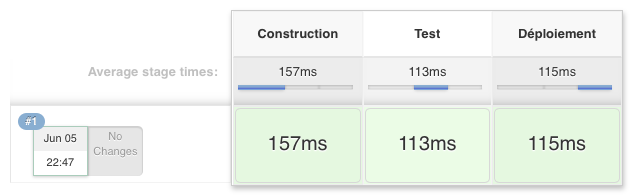
\includegraphics[scale=0.60]{vueStage.png}}
\caption{Exemple de vue de l'�tat des �tapes en temps r�el}
\end{figure} 


\subsection{Le pipeline as code}
Directement int�gr� au sein de l'outil de d�ploiement continu, le pipeline as code permet de cr�er des scripts qui sp�cifieront l'ordre d'enchainement des �tapes effectu�es au sein du d�ploiement continu \cite{18}. Ce script sera ins�r� au sein d'un Jenkinsfile qui demeure un fichier texte contenant la d�finition du pipeline Jenkins. Il est pr�sent au sein du serveur Jenkins est doit �tre accessible � toute la MOE car il s'agit de l'unique source de description du pipeline utilis� au sein du projet. Le contenu du Jenkinsfile est �crit en Groovy, un langage de script orient� Java. \medbreak

\begin{figure}[!h] 
\centerline{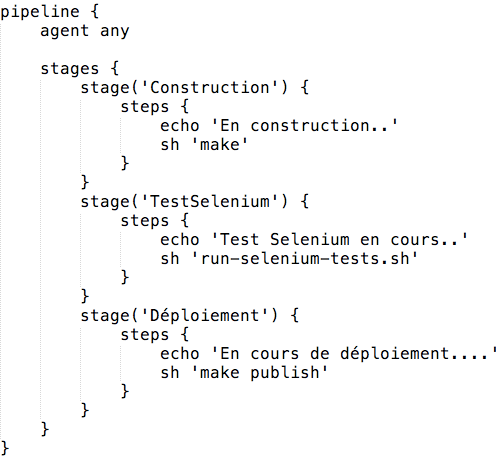
\includegraphics[scale=0.50]{pipelineCodeImg.png}}
\caption{Exemple de script de pipeline}
\end{figure} 

Le script est divis� en diff�rentes parties appell�es "Stage" qui d�signent les �tapes importantes du d�roulement du script. Un stage peut �tre par exemple le build de l'application ou bien le d�ploiement de l'application. A l'int�rieur de ces stages peut se trouver diff�rentes �tapes, appel�es "Steps" � effectuer au sein du stage. Le script peut �galement contenir des commandes, par exemple la commande "sh" qui permet de lancer des scripts lors de l'�xecution du pipeline, ou encore des conditions afin de diriger le d�roulement des �tapes contenues au sein du pipeline.\medbreak 


\chapter{Proposition}
\section{Am�lioration de la recette fonctionnelle d'une application}

Effectu�e manuellement, la recette fonctionnelle d'une application peut s'av�rer longue et fastidieuse, notamment si l'application est r�guli�rement mise �jour, les tests devant �tre effectu�s de mani�re r�guli�re au fur et �mesure des mises � jour. Elle peut donc �tre source de perte de temps et surtout repr�senter un co�t non n�gligeable pour une entreprise.\newline
L'objectif de l'am�lioration de la recette fonctionnelle est donc de r�duire le co�t engendr� par celle-ci. Pour ce faire, il est imp�ratif d'effectuer une automatisation judicieuse des diff�rents cas de tests permettant de couvrir le plus grand nombre de fonctionnalit�s pr�sentes au sein du logiciel.\medbreak
Cependant, il est possible de pousser plus loin l'automatisation de la recette. En effet, m�me si mettre en place des suites de tests automatis�s demeure un r�el progr�s dans le d�roulement des recettes, cette pratique n�c�ssite toutefois des interventions humaines lors de son d�roulement (lancements et suivis des tests) et seul l'AMOA est en connaissance des r�sultats obtenus qu'ils soient positifs ou n�gatifs. L'ensemble de la recette n'est donc pas totalement automatis�. Pour parfaire le processus de recette et ainsi obtenir un r�sultat int�gralement automatis� et accessible �chacun des membres d'une �quipe de projet, int�grer ces tests au sein du processus d'int�gration continue utilis� pour le d�veloppement de l'application est possible et pr�sente diff�rents avantages.\medbreak
En effet, elle permet aux membres de la MOE d'avoir connaissance du r�sultat des tests de l'application au niveau fonctionnel, sans intervention d'assistant � maitrise d'ouvrage, car l'outil d'int�gration continue informe en temps r�el du r�sultat des tests mis en place par ce dernier. Ainsi, ce proc�d� engendre une �conomie de temps non-n�gligeable lors d'une livraison. De plus, elle permet de signaler les r�gressions intervenues lors de chacune des modifications effectu�es au niveau du code sans avoir �v�rifier le comportement de l'application �tant donn� que les tests automatis�s vont v�rifier le comportement de l'application.

\section{Tests automatis�s et int�gration continue}

Gratuit, simple � prendre en main et tr�s fonctionnel, Selenium demeure un outil de choix afin de mettre en place une automatisation des tests fonctionnels. Il permet en effet d'effectuer des tests robustes, jou�s automatiquement de mani�re r�guli�re afin de detecter une regression ou une erreur fonctionnelle. \newline
N�anmoins, Selenium souffre d'un d�faut majeur: s'il est utlis� seul, il ne communique pas les r�sultats des tests effectu�s en dehors de la fen�tre de l'application. En effet, l'outil n'envoie pas de mail, n'affiche pas de notification �l'utilisateur. Le r�sultat d'un test n'est visible qu'en consultant la fen�tre de l'application une fois un test termin�. En outre, il n'indique pas non plus qu'un test est termin�, �l'aide d'une notification par exemple, obligeant ainsi ses utilisateurs � observer r�guli�rement son activit�. \newline
Afin de pallier ce probl�me, il est possible d'int�grer le d�roulement des tests effectu�s avec Selenium au sein de la plateforme d'int�gration continue Jenkins. En effet, ce dernier peut lui m�me ex�cuter les tests Selenium, prendre en compte les r�sultats de ces derniers et en informer rapidement l'�quipe du projet. \medbreak

\subsection{Mise en place des tests automatis�s avec Selenium}
Afin de remplir leur r�le de la mani�re la plus optimale qui soit, les tests automatis�s doivent couvrir un large �ventail de fonctionnalit�s tout en �tant simple �maintenir. \newline
En effet, des tests complexes � maintenir seront vite obsol�tes et donc inutilisables. Cette �tape constitue la plus longue � effectuer et ne demeure r�alisable qu'apr�s la d�veloppement d'une fonctionnalit� car il s'av�re impossible de mettre en place des tests automatis�s d'une fonctionnalit� logicielle tant que celle-ci n'est pas d�velopp�e, les tests �tant bas�s sur le code et l'interface de l'application. \newline
Les tests doivent couvrir le plus large panel de fonctionnalit�s possible. Selenium propose de sauvegarder diff�rents tests sous forme de suite de tests. Il convient donc de diviser chacune des grandes fonctionnalit�s de l'application en suite de tests puis de sous-diviser ces suites en cas de test afin de faciliter la mise �jour ult�rieure de ces tests.

\subsection{Int�gration de Selenium au sein de Jenkins}
L'int�gration de Selenium au sein de Jenkins est rendue possible gr�ce �l'utilisation du plugin Jenkins Selenium. Pour ce faire, il faut proc�der � l'installation du plugin SeleniumHQ au sein de Jenkins. Ce plugin va nous permettre d'ajouter le lancement de tests au sein de la configuration du projet Jenkins. En outre, l'ajout du plugin Selenium HTML report permettra d'afficher les r�sultats des tests effetu�s par Selenium au sein de Jenkins.\newline
Afin de fonctionner, Selenium sera lanc� par Jenkins via l'utilisation de Selenium Remote Control. Ce dernier permet de simuler l'action de Selenium IDE afin d'effectuer les tests. En effet, l'application Selenium IDE n'a nullement besoin d'�tre r�ellement lanc�e par l'utilisateur afin de proc�der � l'ex�cution des tests, Selenium Remote Control agit comme l'application Selenium IDE sans que celle-ci n'ait �t� lanc�e auparavant par un AMOA.

\subsection{Int�gration des tests au sein du pipeline}
Pour cr�er un pipeline sous Jenkins, l'ajout de la suite de plugin Pipeline est indispensable. Celle-ci contient tous les outils permettant d'utiliser les pipelines avec Jenkins en comprenant par exemple l'outil de gestion d'un script de pipeline as code par exemple mais aussi de visualiser le pipeline lors de son utilisation. Le script du pipeline doit sp�cifier l'ordre d'enchainement des �tapes effectu�es au sein de Jenkins et �tre int�gralement pr�sent au sein d'un seul Jenkinsfile par projet. Pour int�grer les tests Selenium au sein du pipeline, il demeure n�cessaire de les int�grer au sein d'un fichier batch sous Windows ou shell sous Macintosh/Linux puis d'inclure leur ex�cution au sein du script du pipeline � l'�tape souhait�e. \medbreak

Afin d'�tre efficace, les pipelines doivent �tre impl�ment�s au sein de Jenkins pour chacun des environnements de travail, de l'environnement de d�veloppement jusqu'�l'environnement de production. En effet, le bon fonctionnement de l'application sur un environnement ne garantit pas que ce sera le cas sur une autre environnement. Les tests automatis�s devront donc �tre execut�s sur l'environnement de recette et de pr�-production afin de permettre de valider le comportement de l'application avant livraison au sein de l'environnement de production.
\medbreak
\begin{figure}[!h] 
\centerline{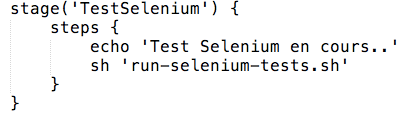
\includegraphics[scale=0.70]{pipelineSelenium.png}}
\caption{Ex�cution des tests Selenium au sein du pipeline}
\end{figure} 
\medbreak

\section{Limites de l'automatisation des tests d'acceptation}
Enjeux important dans l'optique de g�n�rer un gain de temps lors d'une livraison logicielle, l'automatisation des tests fonctionnels souffre aussi de d�fauts certains. Ceux-ci doivent en effet imp�rativement �tre pris en compte par une organisation d�sireuse de mettre en place une automatisation des tests d'acceptation car cette automatisation peut s'av�rer co�teuse ou fastidieuse. \medbreak

\subsection{Une d�marche co�teuse �mettre en place}
L'automatisation de la recette fonctionnelle peut s'av�rer long �mettre en place. En effet, malgr� le faible temps d'ex�cution des tests, leur cr�ation peut repr�senter un co�t non n�gligeable pour l'entreprise car plus l'application comporte de fonctionnalit�s, plus le nombre de test �mettre en place est �lev�. De nombreuses entreprises font donc le choix de r�duire le temps consacr� �la mise en place des tests automatis�s d'acceptation \cite{19}. Il peut donc �tre judicieux de commencer par effectuer une s�lection des tests qui seront � automatiser et les tests trop co�teux � mettre en place seraient ainsi toujours effectu�s manuellement.

\subsection{Le probl�me des changements dans l'interface}

En effet, �tant bas�e sur l'interface graphique d'une application, l'automatisation connait des limites qui peuvent s'av�rer assez lourdes dans le cas de projets r�guli�rement mis �jour \cite{4}. Les tests automatis�s �tant enti�rement bas�s sur l'interface�graphique du programme, si celle-ci vient � changer, les tests s'av�rent totalement obsol�tes. Ils devront �tre enti�rement recr��s. Il demeure donc indispensable de tenir tr�s r�guli�rement �jour les tests dans le cas de changements survenant au niveau de l'interface ou bien si le dom, ou le xpath, des �l�ments est modifi� au niveau du code, ce qui peut repr�senter une certaine perte de temps au sein d'un projet.\medbreak

\subsection{L'obligation de suivre les mises � jour des fonctionnalit�s}
Les tests automatis�s de non-r�gression doivent aussi faire l'objet de mise �jour afin d'�tre fonctionnels. En effet, chacune des fonctionnalit�s impl�ment�es au sein d'une application doit faire l'objet de cr�ation, ou de mises �jour, des tests automatis�s. Ainsi il est imp�ratif de veiller au fait que ceux-ci ne constituent pas une perte de temps trop significative dans le cadre de la bonne avanc�e d'un projet.\newline 
En outre, les changements d'exigences du client peuvent survenir fr�quement, engendrant ainsi une modification du comportement de l'application, attenuant, voir annulant, l'utilit� d'un test ou d'une suite de tests automatis�s parfaitement fonctionnels jusqu'alors. Ainsi, le b�n�fice de l'automatisation des tests d�pend �galement du comportement adopt� par le client. 

\subsection{Seule une �criture tardive demeure possible}
Effectuer les tests d'acceptation n'�tant possible qu'une fois l'application d�velopp�e, il en va de m�me pour leur automatisation. Ainsi, il est impossible d'utiliser une technique de d�veloppement comme le Test Driven Developpement \cite{20} qui consiste � mettre en place les tests unitaires avant de proc�der �l'�criture du code d'une application.\newline
Les tests d'acceptation automatis�s ne peuvent donc pas �tre �crits en amont ou en parall�le du d�veloppement et �tre ainsi utilisables d�s la fin du d�veloppement d'une fonctionnalit�. Le d�marrage de leur �criture ne peut �tre d�but� qu'apr�s la finalisation du d�veloppement ce qui peut repr�senter une perte de temps dans l'avanc�e d'un projet. En effet, selon Cem Kaner \cite{21}, plus les bugs au sein d'une application sont trouv�s tard, plus le co�t de correction est �lev� et le temps pass� ��crire les tests retarde la recherche des bugs au sein de l'application. Ainsi, la mise en place des tests automatis�s peut g�n�rer une perte de temps pour le projet.


\chapter{Conclusion}
Un projet de d�veloppement informatique est compos� de nombreuses phases occupant chacune des parties prenantes par des t�ches diverses et vari�es. Parmi elles, les tests d'acceptation bas�s sur l'interface graphique d'une application constituent une �tape cl� dans l'avanc�e du d�veloppement logiciel car, en plus de permettre d'effectuer la validation d'une livraison applicative, ils permettent de d�tecter rapidement les r�gressions ou probl�mes concernant les fonctionnalit�s d'une application. \medbreak
La recette logiciel, phase du projet durant laquelle l'ensemble des tests d'acceptation est ex�cut�, s'av�re indispensable afin de valider une livraison de nouvelles fonctionnalit�s ou de correctifs via une mise � jour logicielle. Toutefois, une recette effectu�e manuellement peut s'av�rer longue et fastidieuse, g�n�rant un co�t non n�gligeable pour une entreprise. C'est pourquoi nous avons propos� de proc�der � son automatisation afin d'optimiser son efficacit� en mati�re de temps n�cessaire � son d�roulement. Nous avons pu proposer diff�rents outils qui peuvent �tre utilis�s afin de proc�der � une am�lioration de la recette fonctionnelle. Notamment en ce qui concerne l'automatisation des tests d'acceptation ainsi qu'� l'insertion de l'�tape d'ex�cution des tests au sein du processus d'int�gration continue.\medbreak
Nous avons pu voir que l'automatisation des tests est rendue possible gr�ce � l'utilisation d'outils tels que Selenium qui permettent d'automatiser les actions des utilisateurs au sein de l'application. Ainsi, nous avons mis en place l'automatisation des cas d'utilisation afin de pouvoir les simuler en permanence, nous permettant ainsi de valider une livraison mais aussi de d�tecter rapidement une anomalie ou une regression si un test venait � �chouer. Afin d'accro�tre davantage le d�roulement de la recette, nous avons fait le choix d'int�grer ces cas de tests au sein du processus d'int�gration continue gr�ce au pipeline as code propos� par Jenkins. Celui-ci nous a permis de scripter l'enchainement des �tapes existantes au sein de l'int�gration continue. Ainsi, les tests automatis�s peuvent �tre ex�cut�s de mani�re r�guli�re afin de valider une modification dans le code ou bien d'avertir lors de la d�tection d'une anomalie. \newline
Par l'utilisation combin�e de ces outils, le travail de l'AMOA et de la MOE sont ainsi li�s au sein de l'int�gration continue et la recette fonctionnelle peut s'ex�cuter lors de chacune des modifications du code source de l'application. \medbreak
Bien que la mise en place de l'automatisation de la recette fonctionnelle peut constituer une d�marche co�teuse pour une entreprise, proc�der � cette automatisation � l'aide des outils que nous avons d�crits demeure un proc�d� efficace � moyen terme afin d'accro�tre la d�tection des anomalies au sein d'une application et ainsi acc�l�rer la validation d'une livraison de mise � jour. 

\begin{thebibliography}{9}
    \bibitem{1}
Fred D. Davis, Viswanath Venkatesh (2004), Toward Preprototype User Acceptance Testing of New Information Systems: Implications for Software Project Management

   \bibitem{2}
B�rge Haugset, Geir Kjetil (2001), HanssenAutomated Acceptance Testing: a Literature Review and an Industrial Case Study

   \bibitem{3}
Roy W. Miller, Christopher T. Collins (2001), Acceptance Testing

    \bibitem{4}
Malte Finsterwalder (2001), Automating Acceptance Tests for GUI Applications in an Extreme Programming Environment

    \bibitem{5}
Emil Borjesson, Robert Feldt (2012), Automated System Testing using Visual GUI Testing Tools: A Comparative Study in Industry

    \bibitem{6}
Sean Stolberg (2009), Enabling Agile Testing Through Continuous Integration

    \bibitem{7}
Int�gration continue, \newline http://igm.univ-mlv.fr/~dr/XPOSE2010/Lecharpentier\_Jenkins/purpose.html

    \bibitem{8}
http://www.seleniumhq.org/docs/

    \bibitem{9}
http://sikulix-2014.readthedocs.io/en/latest/index.html

    \bibitem{10}
https://a9t9.com/kantu/docs

    \bibitem{11}
https://sahipro.com/docs/introduction/index.html

    \bibitem{12}
HP - Unified Functional Testing, https://saas.hpe.com/fr-fr/software/uft

    \bibitem{13}
Jenkins, https://wiki.jenkins-ci.org/display/JENKINS/Meet+Jenkins

    \bibitem{14}
Bamboo, https://fr.atlassian.com/software/bamboo/features

    \bibitem{15}
TravisCI, https://travis-ci.org/

    \bibitem{16}
CircleCI, https://circleci.com/features/

    \bibitem{17}
Pipeline Jenkins, https://jenkins.io/solutions/pipeline/

    \bibitem{18}
Pipeline as Code, https://jenkins.io/doc/book/pipeline/

    \bibitem{19}
Zhen Ming Jiang,Emad Shihab, Ahmed E. Hassan, Alberto Avritzer, Parminder Flora (2010), An Industrial Case Study on Speeding up User Acceptance Testing by Mining Execution Logs

    \bibitem{20}
Martin Fowler (2005), Test Driven Developement, https://martinfowler.com/bliki/TestDrivenDevelopment.html

    \bibitem{21}
Sam Kaner (1997), Improving the Maintainability of Automated Test Suites


\end{thebibliography}


\end{document}
